The methodology that provided the best results for this assignment counted the the pixels that exceeded an arbitrarily chosen threshold value of 128. The maximum gray scale intensity being 255, this value is the midpoint of the intensity range. This count was subtracted from the mean value of counts from all images in the dataset and finally squared. This choice of anomaly score generation proved to be reasonable. The results are presented later in the paper. The remainder of this section will provide graphical details of the algorithm in action.

An example of two handwriting samples is shown as images in Figure 1 and Figure 2. These images were produced using the imshow function from the matplotlib python library.


\begin{center}
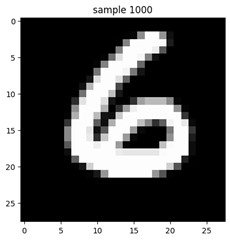
\includegraphics[width=0.25\textwidth]{./images/image1.png}
\captionof{figure}{Handwriting Sample 1000}
\label{fig:sample1}
%\caption{Handwriting Sample 1000}
\end{center}



\begin{center}
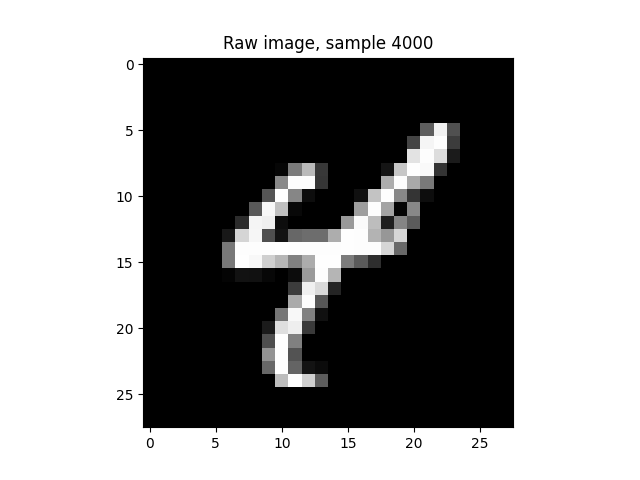
\includegraphics[width=0.25\textwidth]{./images/image2.png}
\captionof{figure}{Handwriting Sample 4000}
\label{fig:sample2}
\end{center}



The first step is producing a thresholded image of each sample as. Experiment 1000 resulted in 615 black pixels and 169 white pixels. Experiment 4000 resulted in 705 black pixels and 79 white pixels.
\begin{center}
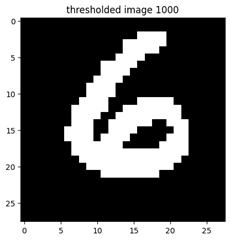
\includegraphics[width=0.25\textwidth]{./images/image3.png}
\captionof{figure}{Threshold set to 128 of handwriting sample 1000}
\label{fig:sample3}
\end{center}

\begin{center}
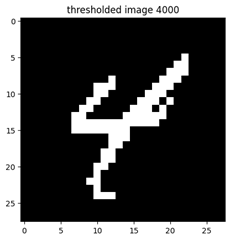
\includegraphics[width=0.25\textwidth]{./images/image4.png}
\captionof{figure}{Threshold set to 128 of handwriting sample 4000}
\label{fig:sample4}
\end{center}


Then a mean image is produced to generate the mean count.
The count of white pixels for the thresholded mean image is 38.
The next step requires subtracting the experiment data from the mean data. The graphical results are shown in the following images.

Now that the subtraction of the experiment image and the mean image has occurred, the resultant value is squared.
